% Template for PLoS
% Version 3.2 March 2016
%
% % % % % % % % % % % % % % % % % % % % % %
%
% -- IMPORTANT NOTE
%
% This template contains comments intended 
% to minimize problems and delays during our production 
% process. Please follow the template instructions
% whenever possible.
%
% % % % % % % % % % % % % % % % % % % % % % % 
%
% Once your paper is accepted for publication, 
% PLEASE REMOVE ALL TRACKED CHANGES in this file 
% and leave only the final text of your manuscript. 
% PLOS recommends the use of latexdiff to track changes during review, as this will help to maintain a clean tex file.
% Visit https://www.ctan.org/pkg/latexdiff?lang=en for info or contact us at latex@plos.org.
%
%
% There are no restrictions on package use within the LaTeX files except that 
% no packages listed in the template may be deleted.
%
% Please do not include colors or graphics in the text.
%
% The manuscript LaTeX source should be contained within a single file (do not use \input, \externaldocument, or similar commands).
%
% % % % % % % % % % % % % % % % % % % % % % %
%
% -- FIGURES AND TABLES
%
% Please include tables/figure captions directly after the paragraph where they are first cited in the text.
%
% DO NOT INCLUDE GRAPHICS IN YOUR MANUSCRIPT
% - Figures should be uploaded separately from your manuscript file. 
% - Figures generated using LaTeX should be extracted and removed from the PDF before submission. 
% - Figures containing multiple panels/subfigures must be combined into one image file before submission.
% For figure citations, please use "Fig" instead of "Figure".
% See http://journals.plos.org/plosone/s/figures for PLOS figure guidelines.
%
% Tables should be cell-based and may not contain:
% - tabs/spacing/line breaks within cells to alter layout or alignment
% - vertically-merged cells (no tabular environments within tabular environments, do not use \multirow)
% - colors, shading, or graphic objects
% See http://journals.plos.org/plosone/s/tables for table guidelines.
%
% For tables that exceed the width of the text column, use the adjustwidth environment as illustrated in the example table in text below.
%
% % % % % % % % % % % % % % % % % % % % % % % %
%
% -- EQUATIONS, MATH SYMBOLS, SUBSCRIPTS, AND SUPERSCRIPTS
%
% IMPORTANT
% Below are a few tips to help format your equations and other special characters according to our specifications. For more tips to help reduce the possibility of formatting errors during conversion, please see our LaTeX guidelines at http://journals.plos.org/plosone/s/latex
%
% For inline equations, please be sure to include all portions of an equation in the math environment.  For example, x$^2$ is incorrect; this should be formatted as $x^2$ (or $\mathrm{x}^2$ if the romanized font is desired).
%
% Do not include text that is not math in the math environment. For example, CO2 should be written as CO\textsubscript{2} instead of CO$_2$.
%
% Please add line breaks to long display equations when possible in order to fit size of the column. 
%
% For inline equations, please do not include punctuation (commas, etc) within the math environment unless this is part of the equation.
%
% When adding superscript or subscripts outside of brackets/braces, please group using {}.  For example, change "[U(D,E,\gamma)]^2" to "{[U(D,E,\gamma)]}^2". 
%
% Do not use \cal for caligraphic font.  Instead, use \mathcal{}
%
% % % % % % % % % % % % % % % % % % % % % % % % 
%
% Please contact latex@plos.org with any questions.
%
% % % % % % % % % % % % % % % % % % % % % % % %

\documentclass[10pt,letterpaper]{article}
\usepackage[top=0.85in,left=2.75in,footskip=0.75in]{geometry}

% Use adjustwidth environment to exceed column width (see example table in text)
\usepackage{changepage}

% Use Unicode characters when possible
\usepackage[utf8x]{inputenc}

% textcomp package and marvosym package for additional characters
\usepackage{textcomp,marvosym}

% fixltx2e package for \textsubscript
\usepackage{fixltx2e}

% amsmath and amssymb packages, useful for mathematical formulas and symbols
\usepackage{amsmath,amssymb}

% for more precise float control
\usepackage{float}

% for \FloatBarrier
\usepackage{placeins}

% cite package, to clean up citations in the main text. Do not remove.
\usepackage{cite}

% Use nameref to cite supporting information files (see Supporting Information section for more info)
\usepackage{nameref,hyperref}

% line numbers
\usepackage[right]{lineno}

% degree symbols
\usepackage{gensymb}

% ligatures disabled
\usepackage{microtype}
\DisableLigatures[f]{encoding = *, family = * }

% Remove comment for double spacing
\usepackage{setspace} 
\doublespacing

%ORCID icons
%\usepackage{fontspec}
%\newfontfamily{\AI}{academicons.ttf}
\usepackage{academicons}
\usepackage{xcolor}
\definecolor{orcidlogocol}{HTML}{A6CE39}

% Text layout
\raggedright
\setlength{\parindent}{0.5cm}
\textwidth 5.25in 
\textheight 8.75in

% Bold the 'Figure #' in the caption and separate it from the title/caption with a period
% Captions will be left justified
\usepackage[aboveskip=1pt,labelfont=bf,labelsep=period,justification=raggedright,singlelinecheck=off]{caption}
\renewcommand{\figurename}{Fig}

% Use the PLoS provided BiBTeX style
\bibliographystyle{plos2015}

% Remove brackets from numbering in List of References
\makeatletter
\renewcommand{\@biblabel}[1]{\quad#1.}
\makeatother

% Leave date blank
\date{}

% Header and Footer with logo
\usepackage{lastpage,fancyhdr,graphicx}
\usepackage{epstopdf}
\pagestyle{myheadings}
\pagestyle{fancy}
\fancyhf{}
\setlength{\headheight}{27.023pt}
%\lhead{\includegraphics[width=2.0in]{PLOS-Submission}}
\rfoot{\thepage/\pageref{LastPage}}
\renewcommand{\footrule}{\hrule height 2pt \vspace{2mm}}
\fancyheadoffset[L]{2.25in}
\fancyfootoffset[L]{2.25in}
% \lfoot{\sf PLOS}

%% Include all macros below

% for easy scientific notation
\providecommand{\e}[1]{\ensuremath{\times 10^{#1}}}
\newcommand{\ipsum}{{\bf IPSUM}}

%for supplemental figures
\newcommand{\beginsupplement}{%
        \setcounter{table}{0}
        \renewcommand{\thetable}{S\arabic{table}}%
        \setcounter{figure}{0}
        \renewcommand{\thefigure}{S\arabic{figure}}%
     }

%% END MACROS SECTION

\begin{document}
\vspace*{0.2in}

% Title must be 250 characters or less.
\begin{flushleft}
{\Large
\textbf\newline{Staphylococcal Smooth Biofilm Morphology on Organotypic Human Keratinocyte Culture is Dependent on \textit{agrA}} % Please use "title case" (capitalize all terms in the title except conjunctions, prepositions, and articles).
}
\newline
% Insert author names, affiliations and corresponding author email (do not include titles, positions, or degrees).
\\
Daniel W. Chan\textsuperscript{\dag} \href{https://orcid.org/0000-0002-8082-2316}{\textcolor{orcidlogocol}{\aiOrcid}},
Juliane Bubeck Wardenburg\textsuperscript{1,2*} \href{https://orcid.org/0000-0002-2755-3348}{\textcolor{orcidlogocol}{\aiOrcid}}
\\
\bigskip
\textbf{1} Dept. of Microbiology, University of Chicago, Chicago, IL, USA
\\
\textbf{2} Dept. of Pediatrics, University of Chicago, Chicago, IL, USA
\\
\bigskip

% Insert additional author notes using the symbols described below. Insert symbol callouts after author names as necessary.
% 
% Remove or comment out the author notes below if they aren't used.
%
% Primary Equal Contribution Note
%\Yinyang These authors contributed equally to this work.

% Additional Equal Contribution Note
% Also use this double-dagger symbol for special authorship notes, such as senior authorship.
%\ddag These authors also contributed equally to this work.

% Current address notes
%\textcurrency Current Address: Dept/Program/Center, Institution Name, City, State, Country % change symbol to "\textcurrency a" if more than one current address note
% \textcurrency b Insert second current address 
% \textcurrency c Insert third current address

% Deceased author note
%\dag Deceased

% Group/Consortium Author Note
%\textpilcrow Membership list can be found in the Acknowledgments section.

% Use the asterisk to denote corresponding authorship and provide email address in note below.
* jbubeck@wustl.edu
\dag danny@danwchan.ca

\end{flushleft}
% Please keep the abstract below 300 words
\section*{Abstract}
Although \textit{Staphylococcus aureus} is known to cause a variety of diseases and thus is a target of many theraputics, for a set of colonized individuals it lives on the human keratinized epidermis without causing disease.
There have been preliminary indications in the literature that colonization involves establishment of a bacterial colony which is protected by a biofilm-like structure.
In this study, we used an organotypic model of human keratinized epithelium \textit{in vitro} and showed it can be colonized for up to 72 hours with \textit{S. aureus} USA300 without compromising normal staining of the granular and suprabasal layers or water permeability.
Bacteria formed colonies covered in a smooth extracellular matrix.
We then tested the effect of mutations in \textit{atl}, \textit{agrA}, 
%\textit{hla},
\textit{icaA}, and \textit{srtA} on colony morphology.
An \textit{agrA}\textsubscript{C123F} mutant demonstrated a slight growth defect and lacked the smooth matrix compared to wild-type.
Unike the phenotype on organitypic cell culture, the mutant phenotype in a model of biofilm production on plastic suggested more biofilm material by crystal violet staining.
However, scanning electron microscopy did not detect the production of extracellular matrix in the plastic model.

% Please keep the Author Summary between 150 and 200 words
% Use first person. PLOS ONE authors please skip this step. 
% Author Summary not valid for PLOS ONE submissions.   
%\section*{Author Summary}

\linenumbers

% Use "Eq" instead of "Equation" for equation citations.
\section*{Introduction}

\textit{Staphylococcus aureus} is a gram positive coccus long known to colonize various sites of the human body~\cite{miko_high_2012,williams_healthy_1963,mermel_methicillin-resistant_2011}.
Human carriage of \textit{S. aureus} has been associated with an increased risk of disease~\cite{wertheim_risk_2004}.
In some cases, disease has been directly linked to a colonizing strain~\cite{von_eiff_nasal_2001, toshkova_significance_2001}.
The anterior nares is often cited as the location of \textit{S. aureus} carriage, but as early as 1946 it was appreciated that \textit{S. aureus} can be found at several sites on the human body~\cite{williams_skin_1946}.
Common sites of colonization are the anterior nares, the inguinal fold, and perineum all of which can be characterized by occluded keratinized epithelium.
Understanding of staphylococcal skin colonization provides insights into the natural history of the organism during the homeostatic prelude to infection.

To establish colonization on the skin, bacteria must interact with the outermost layer of the keratinized epidermis, a dry and slightly acidic layer of enucleated cells called the stratum corneum.
Experimental modeling of the stratum corneum \textit{in vitro} requires the use of complex cell culture techniques primarily used in dermatology studies~\cite{nolte_development_1993}.
In homeostatic conditions, it is thought that lipids in the stratum corneum prevent the diffusion of substances to the granular layer~\cite{elias_epidermal_1983} which can be marked by the presence of loricrin~\cite{hohl_expression_1993}.
The granular layer contains the eponymous keratohyaline granules that positively stain with haemoatoxylin and represent precursor cross-linked proteins of the stratum corneum~\cite{matoltsy_desmosomes_1975}.
Below the granular layer is the stratum spinosum and then the proliferative stratum basale.
Suprabasal layers in organotypic keratinocyte culture can be marked by cytokeratin 10~\cite{stark_organotypic_1999}.
Each layer of the epidermis is derived from the one below.
The deepest layer at the interface of the dermis is the stratum basale made of proliferative cells.
As they differentiate, they form a barrier that renews itself outwards culminating in the sloughing off of desquamated corneocytes from the stratum corneum.

Despite the permeability barrier and shedding, skin microbiota have been observed on and within the stratum corneum of the human skin~\cite{malcolm_demonstration_1980}.
There is evidence that staphylococci live in colonies in this environment~\cite{ten_broeke-smits_hair_2010, nakatsuji_microbiome_2013}.
We hypothesize that given the harsh environment, genetic factors mediating the growth and development of biofilms will allow \textit{S. aureus} to proliferate on the skin surface.
Formation of biofilm in \textit{S. aureus} is thought to involve many genetic factors which differ between strains.
Selected factors are briefly mentioned as follows.
The quorum sensing \textit{agr} locus is expressed in flow-cell biofilms and is reported to upregulate proteases that govern bacterial release~\cite{periasamy_how_2012, boles_agr-mediated_2008, yarwood_quorum_2004}.
Sortase (\textit{srtA}) is a transpeptidase which has been shown to be required for static-well biofilm formation in some strains governed by its substrates~\cite{oneill_novel_2008}.
The intracellular adhesion locus (\textit{ica}) described first in \textit{S. epidermidis}~\cite{mack_intercellular_1996} has also been found to influence \textit{S. aureus} static-well biofilm formation by formation of extracellular polysaccaride~\cite{cramton_intercellular_1999}.
Lastly, the major autolysin \textit{atl} is reported to be required for static-well biofilm formation, possibly by cytosolic protein release or genomic DNA release~\cite{bose_contribution_2012,foulston_extracellular_2014,ranjit_staphylococcus_2011}.

In this study, we reduce the complex environmental conditions of the keratinized epithelium to an \textit{in vitro} model of primary human keratinocytes grown at the air-liquid interface, referred to as organotypic keratinocyte culture or rafts~\cite{simpson_rna_2010}.
These rafts lack indigenous microbiota, professional immune cells and habitual human behaviour all of which may impact bacterial growth, however the rafts provide a reductionist model system in which to study the interaction of bacteria with the stratum corneum.
Raft models have been shown previously to support the growth of bacteria~\cite{breij_three-dimensional_2012, holland_microbial_2008, reijer_detection_2016}.
We were interested in bacterial genetic factors governing this interaction and investigated the colony morphology and growth of various \textit{S. aureus} biofilm mutants on the rafts.
The \textit{agrA}\textsubscript{C123F} mutant showed a smooth biofilm phenotype by scanning electron microscopy on the rafts but form low levels of biofilm in a microtiter plate.
In an opposite manner, $\Delta$\textit{atl} mutants show no signs of biofilm when observed by scanning electron microscopy on rafts while forming high levels of biofilm as measured by the accumulation of crystal violet in a microtier plate.

\section*{Materials and Methods}

\subsection*{Bacterial Strains and Growth Conditions}
\textit{E. coli} DH5$\alpha$ or DC10B was grown in LB media (Sigma L3022) with 100$\mu$g/mL of ampicillin or 15$\mu$g/mL chloramphenicol as required for plasmid maintenance.
\textit{S. aureus} USA300 or RN4220 was grown in TSB media (Remel R455054) with 10$\mu$g/mL chloramphenicol as required.
Table~\ref{table1} contains an annotated list of strains, plasmids and primers used in this study.
%\textit{hla::erm} was generated as previously described~\cite{bubeck_wardenburg_poring_2007}.
\textit{icaA::erm} and \textit{srtA::erm} were made by growing corresponding transposon insertion mutants of \textit{S. aureus} Newman generated in Bae et al.~\cite{bae_staphylococcus_2004} which contained the mutation of interest in a 50:50 mixtures of TSB and LB supplemented with 5mM CaCl\textsubscript{2} to early log (OD\textsubscript{660} = 0.3-0.5) then lysing with bacteriophage $\Phi$85.
Supernatant was cleared by centrifugation (7000g, 40 minutes) and precipitated in PEG 8000.
Overnight cultures of USA300 supplemented with CaCl\textsubscript{2} were infected at 0.1 MOI for 15 mins then phage adsorption was arrested by the addition of sodium citrate to a concentration of 40mM and 3 subsequent washes in cold 40mM sodium citrate.
Transductants were selected on TSB agar containing 40mM sodium citrate and 150$\mu$g/mL erythromycin and confirmed by PCR.
$\Delta$\textit{atl} and \textit{agrA}\textsubscript{C123F} were made according to the methods outlined in Monk et al.~\cite{monk_transforming_2012} with pIMAY-atlKO and pIMAY-agrAC123F respectively.

\subsection*{Plasmid Construction}
To construct pIMAY-atlKO for the generation of USA300 $\Delta$\textit{atl} two flanking segments of the \textit{atl} locus were amplified from the USA300 genome using atl\_lf\_R2, atl\_lf\_F, atl\_rf\_R, atl\_rf\_F.
The fragments were used in a spliced overlap extension (SOE) PCR.
The resulting fragment from SOE PCR contained approximately 1.5kB upstream and downstream of the \textit{atl} start and stop codon respectively and was cloned by restriction digest and ligation into the pIMAY backbone.
pIMAY-agrAC123F for the generation of USA300 \textit{agrA}\textsubscript{C123F} was constructed by amplifying the agrA gene along with 1.5kb upstream and downstream from USA300 using primers with restriction enzyme cut sites at the 5' ends, atl\_stitch\_F and atl\_stitch\_R.
This fragment was cloned into pIMAY and site directed mutagenesis was performed to create the G\textgreater T mutation.
The construct used to complement the \textit{agrA}\textsubscript{C123F} mutation is based on the one used in Peng et. al. where \textit{agrA} expression was driven from the endogenous P1 promoter directly upstream~\cite{peng_cloning_1988}.
The fragment was amplified by PCR for cloning into pOS1 using agrA\_F\_RN\_pst and agrA\_R\_RN\_eco then cloned by restriction digestion.
PCR on single colonies was used to pick candidates for which were confirmed by Sanger sequencing.

% Place tables after the first paragraph in which they are cited.
\begin{table}[!ht]
\begin{adjustwidth}{-2.25in}{0in} % Comment out/remove adjustwidth environment if table fits in text column.
\centering
\caption{
{\bf Strains, plasmids and oligonucleotides used in this study}}
\begin{tabular}{|l|l|l|}
\hline
{ } & {\bf Description} & {\bf Reference/Source}\\ \hline
\multicolumn{3}{|l|}{\bf Strains}\\ \hline
DC10B & strain allowing bypass of \textit{S. aureus} restriction barrier, $\Delta$\textit{dcm} & \cite{monk_transforming_2012}\\ \hline
DH5$\alpha$ & laboratory cloning strain & Invitrogen\\ \hline
RN4220 & \textit{sau1 hsdR} mutant allowing bypass of \textit{S. aureus} restriction barrier & \cite{nair_whole-genome_2011}\\ \hline
Newman & laboratory strain database & \cite{wardenburg_surface_2007}\\ \hline
Newman \textit{agrA::erm} & laboratory strain database & \cite{wardenburg_surface_2007}\\ \hline
LAC & laboratory strain database & \cite{bubeck_wardenburg_poring_2007}\\ \hline
LAC \textit{agrA::erm} & transduced from Pheonix library & this study\\ \hline
LAC \textit{agrA}\textsubscript{C123F} & \textit{agrA} allele exchanged for that of 22251 & this study\\ \hline
LAC $\Delta$\textit{atl} & in frame deletion of \textit{atl} & this study\\ \hline
%LAC \textit{hla::erm} & laboratory mutant & \cite{bubeck_wardenburg_poring_2007}\\ \hline
LAC \textit{icaA::erm} & transduced from Pheonix library & this study\\ \hline
LAC \textit{srtA::erm} & transduced from Pheonix library & this study\\ \hline
3636 &  & \cite{deleo_molecular_2011}\\ \hline
11515 & EMRSA-16 & \cite{deleo_molecular_2011}\\ \hline
21203 & \textit{hla}\textsubscript{STOP} \textit{agrC}\textsubscript{G55R} & \cite{deleo_molecular_2011}\\ \hline
21247 & NRS112, MN-8 & \cite{deleo_molecular_2011}\\ \hline
22251 & 65-20, \textit{agrA}\textsubscript{C123F} & \cite{deleo_molecular_2011}\\ \hline
\multicolumn{3}{|l|}{\bf Plasmids}\\ \hline
pIMAY & allelic replacement vector, built using pKOR & \cite{monk_transforming_2012}\\ \hline
pIMAY-atlKO & to create clean deletion of \textit{atl} & this study\\ \hline
pIMAY-agrAC123F & containing the C123F allele of \textit{agrA} & this study\\ \hline
pOS1 & \textit{E.coli}-\textit{S. aureus} shuttle vector & \cite{schneewind_cell_1993}\\ \hline
pOS1 \textit{agrA} & to complement \textit{agrA} & this study\\ \hline
\multicolumn{3}{|l|}{\bf Oligonuclotides}\\ \hline
pos1\_seq2\_F & GCTTCCGGCTCGTATGTTGTG & this study\\ \hline
pos1\_seq2\_R & GCACCGAAAGCGGATAAC & this study\\ \hline
agrA\_F\_RN\_pst & TGTTATCTGCAGCTGGCCTACGTGATTATTTC & this study\\ \hline
agrA\_R\_RN\_eco & TGTTCGAATTCACGCGTCATATTTAATTTTG & this study\\ \hline
agrA\_pimay\_F\_ecoRI & ATGTAGAATTCAGATGACATGCCTGGCCTAC & this study\\ \hline
agrA\_pimay\_R\_sacI & ATGTTGAGCTCGTGTAGATGTATCAAAAGTG & this study\\ \hline
agrA\_C123F\_F & GAACTCGAATTATAGACTTTTTAGAAACTGCACATAC & this study\\ \hline
agrA\_C123F\_R & GTATGTGCAGTTTCTAAAAAGTCTATAATTCGAGTTC & this study\\ \hline
atl\_lf\_f & GCGTGATCAAAAACCATAACG & this study\\ \hline
atl\_lf\_r2 & GGAGTAATAAATAGAATGGCGAAATAAGCAACATGAACATAGGAT & this study\\ \hline
atl\_rf\_f & CGCCATTCTATTTATTACTCC & this study\\ \hline
atl\_rf\_r & GATGGTGCATGTTATATTTTAGCC & this study\\ \hline
atl\_stitch\_f & ATTATTGAGCTCACGCAAATACTGGGTTAAAAGG & this study\\ \hline
atl\_stitch\_r & ATTATTGGTACCTGATGAAAATGGCATTACCG & this study\\ \hline
\end{tabular}
%\begin{flushleft} Table notes Phasellus venenatis, tortor nec vestibulum mattis, massa tortor interdum felis, nec pellentesque metus tortor nec nisl. Ut ornare mauris tellus, vel dapibus arcu suscipit sed.
%\end{flushleft}
\label{table1}
\end{adjustwidth}
\end{table}

\subsection*{Cell culture growth conditions}
Primary keratinocytes isolated by chemical digestion and mechancal disruption from de-identified neonatal foreskins by the Northwestern University Skin Disease Research Core (NU-SDRC).
They were transported in 75cm\textsuperscript{2} tissue culture flasks filled with M154 media (Thermo-Fisher M154CF500) supplemented with 0.07mM CaCl\textsubscript{2}, Human Keratinocye Growth Supplement (Thermo-Fisher S0015) and gentamicin-amphotericin solution (Thermo-Fisher R01510).
Antibiotics were only used for the first passage of the cells from fresh or frozen, then media without antibiotics were used.
Frozen cell stocks were stored in 10\% DMSO and non-antibiotic containing media at -135\degree C to -190\degree C under vapour phase liquid nitrogen.
Rafts were prepared from either freshly isolated keratinocytes or frozen stocks prepared from 3\e6 passage 2-4 cells.
Passage number 3-7 keratinocytes were used for raft generation.
A mouse fibroblast line, denoted as J23T3 cells, were originally frozen from the NU-SDRC and subsequently maintained in our own lab 
J23T3 cells were grown in DMEM containing with 4.5g/L glucose, glutamine and sodium pyruvate (Corning Cellgro 10-013) supplemented with 10\% fetal bovine serum (Corning Cellgro 35-010-CV, L024-6).
Rafts were grown according to the protocols established by the NU-SDRC as outlined in Simpson et al.~\cite{simpson_rna_2010} by seeding keratinocytes on a collagen plug impregnated with fibroblasts and subsequently lifting to the air-liquid interface which drives differentiation.
The following modifications were made to their protocol:
10x collagen plug resuspension buffer is stored at 4\degree C;
0.75mL of the collagen-fibroblast slurry was used to seed a sterile 24-well plate;
keratinocytes are delivered in 1ml of media to the plugs.
An overview of raft growth and bacteria exposure can be found in Fig~\ref{figS1}A.

\subsection*{Bacterial inoculation of rafts}
For treatment of rafts at the lowest CFU possible, \textit{S. aureus} were grown at an OD$_{660}$ of 0.4-0.5 (Thermo, Genesys 20 Spectrophotometer), washed in autoclaved phosphate buffered saline (PBS) and diluted to the appropriate CFU/mL concentration (empirically determined to be approximately a 1\e{-4} dilution) in artificial sweat media.
Artificial sweat media was prepared according to the protocol in Harvey et al~\cite{harvey_formulation_2010} with the following modifications:
sulfur was omitted and the concentration of riboflavin was reduced to 7.53\e{-2} because of solubility issues;
the concentration of nicotinic acid was reduced to 5.05\e{-1}g/L because it strongly inhibited growth/attachment of \textit{S. aureus}.
3$\mu$L of diluted bacteria were applied to the rafts by pipetting and allowed to attach for 3.5 hours.
Typically three drops were placed on the keratinized epidermis, two containing bacteria and one control without bacteria.
The drops were then blotted off with autoclaved chromotography paper (Whatman 3030-392) with care not to touch the surface and the position of the bactera exposed areas were noted on the lid of the tissue culture dish.
Batches of rafts treated with bacteria occasionally became contaminated.
If rafts were compromised they were omitted from the study, and if the majority of rafts were contaminated in a batch the whole study was omitted.

\subsection*{Enumeration of colony forming units from rafts}
Sections of rafts containing bacteria were removed from the surface of the metal grids using forceps and a scalpel sterilized with ethanol.
Typically one bacteria treated section would be transferred to a tube containing 1mL of 0.01\% Triton X-100 diluted in PBS on ice for CFU enumeration.
The remaining section of the rafts, containing a bacteria treated and control treated area, would be flooded with fixative for use in microscopy.
If the exposed areas could not be separated the entire raft was homogenized and the CFU was tagged as "double" which was normalized in analysis. 
Samples for enumeration were homogenized in a rotor stator homoginizer (PRO Scientific, Bio-Gen PRO200) at ~70\% power pulsed 3 times for 5 seconds until the mixture was a pale pink and no large particles of tissue remained.
150$\mu$L of the homogenate was serially diluted in PBS using the rows of a sterile 96-well plate from undiluted to 10\e{-7}.
A multichannel pipette was used to plate 10$\mu$L from each column representing a sample on TSB agar.
The agar plates were incubated for overnight and colonies were enumerated using an hand counter.

\subsection*{Plastic surface biofilm assay}
Overnight staphylococcal cultures were diluted to OD\textsubscript{660} = 0.05 in TSB media containing 5\% glucose.
175$\mu$L of the diluted cultures were added by column to the wells of a 96-well plate (Corning Costar 3585), omitting the outermost wells.
Bacteria were incubated at 37\degree C with a lid in a humidified foam box for 24 hours.
Liquid was removed by quickly inverting over a large beaker of hypochlorite bleach and the wells were washed twice with 200$\mu$L of PBS with drying achieved by tapping on paper towels.
Plates were then dried in a 60\degree C oven for 1 hour before staining the baked material with 50$\mu$L of 0.41\% crystal violet in 12\% ethanol for 5 minutes.
Stain was removed with a pipette and the wells were again washed twice with 200$\mu$L of PBS.
Bound crystal violet was eluted with 50$\mu$L 33\% acetic acid and 25$\mu$L of the eluate was diluted in 100$\mu$L of distilled water in a U-bottom plate for spectrophotometric reading at 595nm (Tecan infinite M200 Pro).
Except for initial inoculation, liquid handling was performed by row and thus normalized optical density is calculated from the (mean) well absorbance of wild type \textit{S. aureus} in each row.

\subsection*{Scanning electron microscopy and sample preparation}
For biofilms grown in 96-well plates, a razor blade and acetone were used to remove material from bottom of the plate until the base of a single well was thin enough to be excised by the razor.
All samples were fixed in 2\% paraformaldehyde, 2\% glutaraldehyde in PBS for 1-3 hours at 37\degree C then overnight at room temperature.
Samples were stored in 70\% ethanol at 4\degree C for up to one month before dehydrating in a series of ethanol washes (2x 80\%, 1x 95\%, 1x 100\% were each used for 15 mins).
The dried rafts were cut under ethanol to an appropriate size for the SEM pin (Ted Pella 16111-9).
Samples were then further dried overnight in 100\% ethanol that was stored with 4\r{A} molecular sieves.
The ethanol was exchanged for hexamethyldisilazane (HMDS) in two grades of HDMS:ethanol (50:50, 100:0) for 15 minutes each, then the final HDMS was removed and replaced with a very small volume of HDMS.
This small amount of HDMS was allowed to evaporate partially covered in the fume hood until completely dry, then samples were mounted on SEM pins using double-sided carbon tape (Ted Pella 16084-3) and sputter coated with 8nm 20/80 platinum/palladium (Ted Pella Cressington 208HR, 40mA).
Prepared pins were stored in an air-tight container with desiccant before imaging on the FEI NanoSEM Nova 230 (5-15kV, 12$\mu$s dwell).

\subsection*{Light microscopy and sample preparation}
For light microscopy, rafts were fixed in 10\% formalin in PBS overnight at room temperature.
Rafts were then stored in 70\% ethanol at 4\degree C before being cut, packed into cassettes.
Nationwide Histology (Veradale, WA) was responsible for paraffin embedding, sectioning (4$\mu$m) and H\&E staining.
Slides were scanned using CRi Pannoramic Scan Whole Slide Scanner and images exported from Pannoramic Viewer version 1.15.4 were processed in Fiji~\cite{schindelin_fiji:_2012}.

\subsection*{Immunofluorescence microscopy and staining}
Unstained 4$\mu$m paraffin sections from Nationwide Histology were baked at 60\degree C for 1 hour then the deparaffinized in xylene (2x washes, 10 minutes) and rehydrated in a series of graded ethanol solutions (95\%, 80\%, 70\%, 50\%, 30\%, water).
Antigen retrieval was performed by heating slides to 95\degree C in 10mM citrate buffer (pH 6.0) for 1 hour then cooling slowly to room temperature.
Slides were blocked for 1 hour in wash buffer (10X: 0.5M Tris-HCl pH 7.6, 1.5M NaCl, 0.5\% Tween 20) with 1:100 human IgG (Thermo 31154) and 10\% goat serum.
Primary antibody was applied in wash buffer with 1\% goat serum and incubated overnight.
Concentrations for each antibody are as follows:
1:50 K10 (LH-2, Chemicon CBL196)
1:100 loricrin (AF62, Covance PRB-145P)
Slides were then washed 3 times before 1:400 goat anti-mouse Alexa488 (A1101) or goat anti-rabbit Alexa594 (A11037) was applied in wash buffer with 1\% goat serum for 1 hour and washed 3 more times.
Mounting media containing DAPI was used (Thermo-Fisher P36935) and slides were allowed to cure for 24h before imaging on the Zeiss Axiovert 200M or the Olympus DSU confocal.
Images were exported from Slidebook version 5/6 and processed in Fiji~\cite{schindelin_fiji:_2012}.

\subsection*{Statistical analysis and figure generation}
Statistics were performed in R packages used can be found in the code. Analysis was written in R~\cite{r_core_team_r:_2015} and annotated in a modified Rmarkdown using RStudio.
HTML reports were compiled for reference. Raw data, code and reports are available from the Open Science Framework~\cite{chan_organotypic_2016}.
Figures were made in Inkscape and can be regenerated by makefile commands in the root folder of this project.

% Results and Discussion can be combined.
\section*{Results}

%PLOS does not support heading levels beyond the 3rd (no 4th level headings).

\subsection*{Organotypic rafts support \textit{S. aureus} growth}

To evaluate the interaction of \textit{S. aureus} USA300 (LAC) with primary human epidermis, we used an organotypic model that recapitulates fully differentiated and stratified human skin~\cite{simpson_rna_2010}.
Staphylococci were applied across a range of inocula to mature organotypic rafts, and assessed for the ability to sustain growth on the tissue.
By 24 hours, initial inocula between 10\textsuperscript{1}-10\textsuperscript{3} all reached a similar density of approximately 10\textsuperscript{8}CFU/raft (Fig~\ref{fig1}A), supported by effect size analysis using the Cliff's delta statistic.

Light microscope evaluation of paraffin embedded H\&E stained sections revealed staphylococcal colonies in close association with the eosin stained stratum corneum as early as 72 hours (Fig~\ref{fig1}B).
The integrity of the stratum granulosum was undisturbed supported by staining for the granular layer marker loricrin (Fig~\ref{fig1}B, red), which forms an unbroken band of positive signal along the raft section corresponding to the cells with haematoxylin stained granules.
The marker cytokeratin 10 (Fig~\ref{fig1}B, green) was used to stain the suprabasal layers of the rafts and the stratum basale can be identified by isolated DAPI staining (Fig~\ref{fig1}B, blue).
Cytokeratin 10 is not excluded from the stratum basale at 120 hours, likely reflecting raft aging, however at this time point the stratum granulosum remained intact (Fig~\ref{fig1}B).
72 hours post treatment was fixed as the primary observational timepoint since it demonstrated the most normal looking cell strata and the \textit{S. aureus} colonies had a distinct compact morphology.

To assess the barrier function of rafts, a water soluble dye called lucifer yellow was applied to \textit{S. aureus} treated rafts and untreated rafts.
Lucifer yellow penetration into the rafts was not altered by the presence of staphylococci relative to PBS treatment alone (Fig~\ref{fig1}C, top panels).
In contrast, deliberate compromise of the barrier by 1\% SDS resulted in disruption of loricrin staining and penetration of the lucifer yellow past the stratum granulosum (Fig~\ref{fig1}C, bottom panel).

% Place figure captions after the first paragraph in which they are cited.

\begin{figure}[!ht]
\begin{adjustwidth}{-2.25in}{0in}
\includegraphics[width=0.85\paperwidth]{Figures/fig1.pdf}
\caption[Characterization of the model with wild type \textit{S. aureus} USA300]{
	\textbf{Characterization of the model with wild type \textit{S. aureus} USA300}
	(A) CFU recovered from rafts after 0 - 120 hours. \textit{p} values calculated using Dunn's post hoc test after passing 0.05 significance threshold in the Kruskall-Wallis multiple comparison test. 95\% confidence intervals of the differences are reported using Cohen's \textit{d} as the effect size. Data pooled from 3 experiments.
	(B) Light microscopy of H\&E stained sections of treated rafts (left panel) and immunofluorescent microscopy of matched sections 4$\mu$m apart stained with DAPI and antibodies against loricrin and cytokeratin 10 (right panel and inserts). Rafts were harvested at 24, 72 and 120 hours. IF microscopy is false coloured using the scheme indicated by the text colour. Scale bars are 100$\mu$m. Images representative of at least 3 experiments.
	(C) Immunofluorescent microscopy of sections from untreated (top and bottom panel) and treated (middle panel) rafts which prior to fixation and harvesting were treated with PBS containing lucifer yellow for 2.5 hours. Sections were further stained with DAPI and loricrin, false coloured by the scheme indicated in the text. Scale bars are 100$\mu$m. Images are representative of at least 2 experiments.}
    \label{fig1}
    \end{adjustwidth}
\end{figure}

\subsection*{The \textit{agrA}\textsubscript{C123F} mutant has defective biofilm formation}

Scanning electron microscopy was used to investigate the colony morphology of \textit{S. aureus} on the organotypic rafts.
Microcolonies formed as soon as 2 hours after blotting off excess liquid.
These colonies grew within 24 hours into larger covered colonies and by 72 hours had a conspicuous smooth extracellular matrix which could be seen pulling away from the edges of individual cocci (Fig~\ref{figS2}).
Extracellular matrix production was interpreted as the formation of a biofilm.

To investigate the origin of the extracellular matrix and perturb the interaction between the \textit{S. aureus} and the raft, bacterial mutants in the USA300 strain were constructed targeting biofilm related genes.
The mutant colonies were imaged using scanning electron microscopy at 72 and 120 hours (Fig~\ref{fig2}, ~\ref{figS3}).
Only the \textit{agrA}\textsubscript{C123F} mutant differed from the appearance of wild-type (Fig~\ref{fig2}, top right panel).
The colonies of this mutant were rough, relatively uncovered and had an undulate margin in contrast to the wild type appearance of smooth, covered colonies and rounder margins (Fig~\ref{fig2}, top left versus top right panel).
Mutant colonies lack the smooth extracellular matrix observed in the wild-type colonies (Fig~\ref{fig2}, top left and right panel, top insert).
The same phenotype was observed in a strain of Newman carrying an \textit{agrA::erm} allele (Fig~\ref{figS4}C).
The mutant strain of USA300 was complemented by an epigenetic plasmid containing \textit{agrA} driven by the P1 promoter which returned the colony morphology back to wild-type (Fig~\ref{fig2}, bottom left panel).
A clinical strain designated 22251 also showed the rough, uncovered phenotype (Fig~\ref{figS5}A, bottom left panel).
22251 carries the \textit{agrA}\textsubscript{C123F} allele and could be complemented by wild type \textit{agrA} to increase growth and promote smooth covered colonies (Fig~\ref{figS5}A, bottom right panel, Fig~\ref{figS5}B).


\begin{figure}[!ht]
\begin{adjustwidth}{-2.25in}{0in}
\includegraphics[width=0.85\paperwidth]{Figures/fig2.pdf}
\caption[Investigation of \textit{S. aureus} USA300 and mutants' colony morphology on the rafts]{
	\textbf{Investigation of \textit{S. aureus} USA300 and mutants' colony morphology on the rafts}
	(A) Scanning electron microscopy of bacterial colonies on the raft surface at 1200x (large left) and 20000x (right inserts) taken at 72 hours. Scale bars are 50$\mu$m and 2$\mu$m respectively. Images are representative of at least 2 experiments.}
    \label{fig2}
    \end{adjustwidth}
\end{figure}

\subsection*{The \textit{agrA}\textsubscript{C123F} mutant has a growth defect on the raft}

The \textit{agrA}\textsubscript{C123F} mutant demonstrated a modest growth defect 72 hours and 120 hours after treatment (Fig~\ref{fig3}).
This defect could be complemented by the P1 promoter driven plasmid copy of \textit{agrA}.
These differences from wild type USA300 were statistically significant by both non-parametric null hypothesis testing and effect size analysis.
The complementing plasmid was also able to increase the growth of strain 22251 (Fig~\ref{figS5}B). 

The $\Delta$\textit{atl} mutant only demonstrated a growth defect at 72 hours (Fig~\ref{figS3}A).
There was no notable change in growth between each of the \textit{icaA::erm}, 
%\textit{hla::erm},
\textit{srtA::erm} mutants and wild type (Fig~\ref{figS3}A).


\begin{figure}[!ht]
\begin{adjustwidth}{-2.25in}{0in}
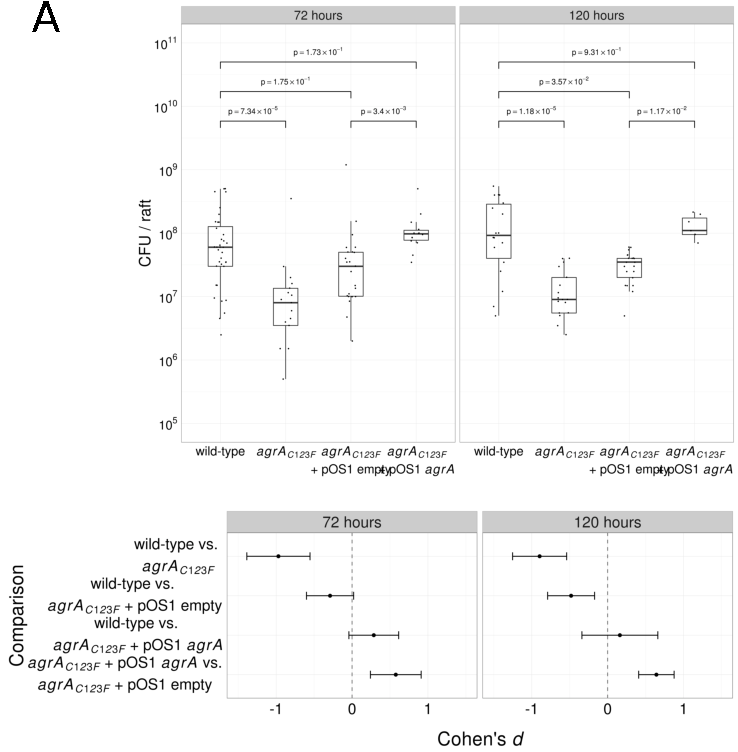
\includegraphics[width=0.85\paperwidth]{Figures/fig3.pdf}
\caption[Investigation of \textit{S. aureus} USA300 and mutants' growth on the rafts]{
	\textbf{Investigation of \textit{S. aureus} USA300 and mutants' growth on the rafts}
	(A) CFU recovered from rafts after 72 and 120 hours. \textit{p} values calculated using Dunn's post hoc test after passing 0.05 significance threshold in the Kruskall-Wallis multiple comparison test. 95\% confidence intervals of the differences are reported using Cohen's \textit{d} as the effect size. Data are pooled from 4 experiments.}
	\label{fig3}
    \end{adjustwidth}
\end{figure}

\subsection*{Biofilm morphology on rafts does not correlate with biofilm on plastic}

The smooth extracellular matrix was absent in the \textit{agrA}\textsubscript{C123F} mutant as observed by SEM, yet the mutant had the highest biofilm signal in the static well assay (Fig~\ref{fig4}A).
This increased static biofilm accumulation was reduced back to wild type in the complemented strain (Fig~\ref{fig4}A).
The assumption of the static well assay is that biofilm material is fixed to the wells, stained with crystal violet and quantified.
To assess the validity of the assumption, we searched for the presence of extracellular matrix on excised well bottoms using the same scanning electron microscopy preparations used to prepare rafts.
Excised wells showed dense aggregates of bacteria adhering to the polypropylene and each other but no evidence of extracellular matrix deposition (Fig~\ref{fig4}B, upper panels).
After washing as per the static well assay method, a layer of bacteria remained adhered to the polystyrene which presumably is stained and quantified by crystal violet (Fig~\ref{fig4}B, lower panels).
The observation that the $\Delta$\textit{atl} mutant had low crystal violet absorbances in the static well assay but showed wild type amounts of smooth extracellular matrix on rafts further supports the difference between the biofilm signal in these models (Fig~\ref{figS3}B,~\ref{figS6}A).
The \textit{atl} and \textit{agrA}\textsubscript{C123F} mutants showed defects in biofilm morphology on raftsby SEM which were opposite from those observed on a plastic substrate by crystal violet absorption.
The differences in the amount of biofilm on plastic were statistically significant by non-parametric null hypothesis testing and effect size analysis using the Cliff's $\Delta$ statistic.
The \textit{icaA::erm} and \textit{srtA::erm} mutants were not significantly different from wild type in biofilm morphology observed by SEM nor from those observed in the static biofilm model on a plastic substrate (Fig~\ref{figS3}B, \ref{figS6}A).


\begin{figure}[!ht]
\begin{adjustwidth}{-2.25in}{0in}
\includegraphics[width=0.85\paperwidth]{Figures/fig4.pdf}
\caption[The \textit{agrA}\textsubscript{C123F} \textit{S. aureus} hyper-biofilm phenotype in 96-wells does not involve extracellular matrix]{
	\textbf{The \textit{agrA}\textsubscript{C123F} \textit{S. aureus} hyper-biofilm phenotype in 96-wells does not involve extracellular matrix}
	(A) Normalized absorbances from a 96-well crystal violet static biofilm assay. \textit{p} values calculated using Dunn's post hoc test after passing 0.05 significance threshold in the Kruskall-Wallis multiple comparison test. 95\% confidence intervals of the differences are reported using Cliff's $\Delta$ as the effect size. Data are pooled from at least 4 experiments.
	(B) Scanning electron microscopy of bacteria fixed before and after washing on a polystyrene surface at 1200x (large) and 20000x (insert). Scale bars are 50$\mu$m and 2$\mu$m respectively. Images are representative of at least 2 experiments.}
    \label{fig4}
    \end{adjustwidth}
\end{figure}

\section*{Discussion}

The experimental system we report here is similar to that reported in Reijer et al. and Holland et al. ~\cite{reijer_detection_2016,holland_microbial_2008}.
Like Reijer et al. but unlike Holland et al. we observe no lag in growth, this can be explained by the use of stationary phase bacteria by Holland et al.
It is interesting to consider the humidified chamber of the tissue culture incubator and how that may contribute to the growth of \textit{S. aureus} on the raft.
Early experiments demonstrated that occluding the skin, thus increasing CO\textsubscript{2} and humidity, like the tissue culture incubator, causes bacterial numbers to increase~\cite{lovell_skin_1945-1}.
The organotypic model only captures the occluded environmental condition and so is limited in its ability to reveal insights on the role of dormant bacteria in the model.

Unlike Holland et al. and Reijer et al. we omitted the use of antibiotics which could confound the study of biofilms~\cite{kaplan_low_2012}, but it is unclear if this was necessary.
Note that even with the use of antibiotics Holland et al. report that at later timepoints the rafts become overgrown with bacteria.
This occurred occasionally during the course of our experiments and we interpret this to reflect the variability of barrier function between rafts, making this model particularly challenging to work with.
However, for the samples taken for histology, the barrier function of the rafts seem intact at 72 hours (Fig~\ref{fig1}BC).
This suggests that most water soluble products from the colonies of S. aureus are not be able to reach granular layer cells unless they use specific transport mechanisms.
Future studies would benefit from batch specific lucifer yellow permeability, raman spectroscopy (for water) or transepidermal water loss assays to control for barrier function variability between each batch, particularly if hypotheses would suggest the diffusion of bacterial products to the lower cell layers.

The functional significance of the smooth matrix encasing these colonies is unknown.
A potential hypothesis is that it is responsible for tight adhesion to the stratum corneum.
Based on the defect in the \textit{agrA}\textsubscript{C123F} growth and its uncovered appearance,  another potential hypothesis is that the matrix provides some sort of protection from growth inhibitory compounds produced by the organotypic model.
Consistent with the understanding that \textit{agrA} is a quorum sensing response regulator the defect in growth manifests at higher densities of bacteria, unlike the defect in growth associated with \textit{atl} which seems most apparent at 72 hours but less so at 120 hours (Fig~\ref{figS3}A).
What is promising for continued used of this model is the previous report of covered colonies observed by SEM on the skin and a distinct pitting from cells that are dislodged from their position~\cite{malcolm_demonstration_1980} also observed in the \textit{in vitro} model (Fig~\ref{fig2}C, bottom right inset).
Also consistent with their observation of colonies on the underside of a stratum corneum surface is the layer of eosin stained material that is particularly notable in the 120 hour H\&E stained picture (Fig~\ref{fig1}B).
The lucifer yellow penetrates the bacterial colony deeply which could be analogous to the channels observed in flow derived biofilms~\cite{periasamy_how_2012}, but it could also indicate that the bacteria grow along water permeable corneocyte junctions.
Malcolm et al. report colonies that are seldom more than two bacteria deep which is unlike what we observe in this model.
Perhaps this reflects the constant shedding of bacteria from movement and presents a further limitation on the model as we have employed it here.

The visual appearance of the extracellular matrix was not dependent on \textit{icaA}, \textit{srtA} or \textit{atl}, which sheds light on the potential composition of the material (Fig~\ref{figS3}A).
The lack of dependence on \textit{icaA} suggests that PNAG is not required for the formation of the smooth covering.
This is consistent with the literature where some strains are reported to form \textit{icaA} independent biofilms~\cite{fitzpatrick_evidence_2005}.
However, a proposed alternative factor named fibronectin binding protein, is \textit{srtA} dependent~\cite{oneill_novel_2008}, but \textit{srtA} is independent of the biofilm morphology formed on rafts (Fig~\ref{figS3}A).
The \textit{atl} mutant addresses another potential biofilm development pathway, that of autolysis and extracellular DNA release~\cite{bose_contribution_2012}.
Since there are multiple genetic factors which may be responsible for eDNA release, the lack of \textit{atl} contribution does not rule out the contribution of this macromolecule to the smooth matrix~\cite{ranjit_staphylococcus_2011}.

It has been shown in static and flow based biofilms that mutations in \textit{agrA} cause the accumulation of biofilm material ~\cite{periasamy_how_2012}.
Presumably this disrupts production of proteases and nucleases which help release biofilm material~\cite{boles_agr-mediated_2008, kiedrowski_nuclease_2011}.
These literature agree with the increase of biofilm accumulation as measured by crystal violet (Fig~\ref{fig4}A) but not with the colony morphology observed by SEM (Fig~\ref{fig2}) which are covered by extracellular material.
However, when the wells used in the crystal violet assay were used for SEM, we observed that, absorbance is more a function of cell adherence than of accumulation of extracellular matrix (Fig~\ref{fig4}B), which supports a hypothesis that factors contributing to biofilm formation under liquid are unlike those for the raft.
\textit{agrA} is known to regulate the production of \textit{hla} which has been implicated in biofilm production~\cite{caiazza_alpha-toxin_2003} which may be responsible for the change in biofilm morphology.
%,but we do not see an effect of \textit{hla} on the covered colony morphology.
Another potential hypothesis is that amyloid aggregations of phenol soluble modulins are responsible for stabilizing the structure of these biofilms~\cite{schwartz_functional_2012}.
Perhaps related to this phenomenon is the observation of filament like biofilm (Fig~\ref{figS3}B, $_\Delta$\textit{atl}).
However, the observation of this texture was unpredictable and seemingly associated randomly with the covered, smooth margin colony morphology.

To rationalize the observations made in this raft model, we think about the staphylococcal niche of the stratum corneum.
Corneocytes do not have a nucleus, thus cannot transcriptionally respond to stimulus, and access to the lower layers is restricted by permeability barriers.
This presents a challenge to the interpretation of existing literature demonstrating effects of \textit{S. aureus} on keratinocytes~\cite{mempel_invasion_2002, menzies_signal_2006, secor_staphylococcus_2011, soong_methicillin-resistant_2015, haugwitz_pore-forming_2006}.
The plethora of reported effects could occur during disease states when bacteria have access to underlying cells, but during colonization we hypothesize there are only interactions with the stratum corneum.
Alternatively, colonization may occur as a constant cycle of invasion and successful defence.
However, the organotypic model cannot be used to test this alternative, it is uniquely poised to study the initial interaction of \textit{S. aureus} with the stratum corneum in relative isolation.
The stratum corneum is an air perfused, slightly acidic, high osmolarity environment.
This is quite unlike the liquid submerged models of biofilm production which may better capture the conditions of implant associated infections.
As expected, the raft colonies with biofilm morphology differ in their genetic requirements from submerged cultures.

\section*{Conclusion}
Organotypic keratinocyte rafts are an unique model to study the interaction between \textit{S. aureus} and a human keratinized epithelium.
When \textit{S. aureus} is grown on this surface it forms colonies encased in a smooth extracellular matrix which is dependent on \textit{agrA} but not \textit{icaA}, \textit{srtA}, 
%\textit{hla}
or \textit{atl}.
Our study suggests that biofilms produced in plastic microtiter dishes have different genetic determinants than those required in the \textit{in vitro} model of the stratum corneum.

\beginsupplement

\section*{Supporting Information}

% Include only the SI item label in the paragraph heading. Use the \nameref{label} command to cite SI items in the text.
\begin{figure}[H]
\begin{adjustwidth}{-2.25in}{0in}
\includegraphics[width=0.85\paperwidth]{Figures/figS1.pdf}
\caption[An visual overview of the standard experimental workflow]{
\textbf{An visual overview of the standard experimental workflow}
This workflow was used for the majority of experiments. Normal human epidermal keratinocytes were obtained fresh from the Northwestern University Skin Disease Research Core or revived from previously obtained stocks stored in liquid N\textsubscript{2}. In contrast to other models of organotypic rafts, antibiotics were only used for the first 1-2 passages in submerged culture (pre raft growth).}
\label{figS1}
\end{adjustwidth}
\end{figure}

\begin{figure}[H]
\begin{adjustwidth}{-2.25in}{0in}
\includegraphics[width=0.85\paperwidth]{Figures/figS2.pdf}
\caption[Fine time course of USA300 colony morphology on rafts]{
\textbf{Fine time course of USA300 colony morphology on rafts} 
	(A) Scanning electron microscopy of bacterial colonies on the raft surface at 1200x (left panel) and 20000x (right panel) taken from 2 - 120 hours. Scale bars are 50$\mu$m and 3$\mu$m respectively. Images are representative of 2 experiments.}
    \label{figS2}
    \end{adjustwidth}
\end{figure}

\begin{figure}[H]
\begin{adjustwidth}{-2.25in}{0in}
\includegraphics[width=0.85\paperwidth]{Figures/figS3.pdf}
\caption[Other tested mutants did not show colony morphology differences despite slight growth differences]{
	\textbf{Other tested mutants did not show colony morphology differences despite slight growth differences}
	(A) CFU recovered from rafts after 72 and 120 hours. \textit{p} values calculated using t-test with non-pooled SD. 95\% confidence intervals of the differences are reported using Cohen's \textit{d} as the effect size. Data are pooled from 4 experiments.
	(B) Scanning electron microscopy of bacterial colonies on the raft surface at 1200x (large left) and 20000x (right inserts) taken at 72 hours. Scale bars are 50$\mu$m and 2$\mu$m respectively. Images are representative of 3 experiments.}
        \label{figS3}
        \end{adjustwidth}
\end{figure}

\begin{figure}[H]
\begin{adjustwidth}{-2.25in}{0in}
\includegraphics[width=0.85\paperwidth]{Figures/figS4.pdf}
\caption[Preliminary indication that an \textit{agrA::erm} mutant of \textit{S. aureus} Newman also has a growth defect and shows lack of smooth extracellular matrix]{
\textbf{Preliminary indication that an \textit{agrA::erm} mutant of \textit{S. aureus} Newman also has a growth defect and shows lack of smooth extracellular matrix}
	(A) CFU recovered from rafts after 72 hours. \textit{p} value calculated using Wilcox signed rank test. Data come from a single experiment.
	Below, confidence interval and effect size expressed as Cliff's $\Delta$.
	(C) Scanning electron microscopy of bacterial colonies on the raft surface at 1200x (large left) and 20000x (right inserts) taken at 72 hours. Scale bars are 50$\mu$m and 2$\mu$m respectively. Images are representative of 2 experiments.}
        \label{figS4}
        \end{adjustwidth}
\end{figure}

\begin{figure}[H]
\begin{adjustwidth}{-2.25in}{0in}
\includegraphics[width=0.85\paperwidth]{Figures/figS5.pdf}
\caption[In a diverse range of strain backgrounds only an \textit{agrA} lesion in \textit{S. aureus} 22251 produces the disrupted extracellular matrix phenotype]{
	\textbf{In a diverse range of strain backgrounds only an \textit{agrA} lesion in \textit{S. aureus} 22251 produces the disrupted extracellular matrix phenotype}
	(A) Scanning electron microscopy of bacterial colonies on the raft surface at 1200x (large left) and 20000x (right inserts) taken at 72 hours. Scale bars are 50$\mu$m and 2$\mu$m respectively. Images are representative of 2 experiments.
	(B) CFU recovered from rafts after 72 and 120 hours. \textit{p} values calculated using t-test with non-pooled SD. 95\% confidence intervals of the differences are reported using Cliff's $\Delta$ as the effect size. Data are pooled from 3 experiments.}
        \label{figS5}
        \end{adjustwidth}
\end{figure}

\begin{figure}[H]
\begin{adjustwidth}{-2.25in}{0in}
\includegraphics[width=0.85\paperwidth]{Figures/figS6.pdf}
\caption[96-well biofilm assay for other mutants of USA300]{
	\textbf{96-well biofilm assay for other mutants of USA300}
	(A) Normalized absorbances from a 96-well crystal violet static biofilm assay. \textit{p} values calculated using Dunn's post hoc test after passing 0.05 significance threshold in the Kruskall-Wallis multiple comparison test. 95\% confidence intervals of the differences are reported using Cliff's $\Delta$ as the effect size. Data are pooled from at least 4 experiments.}
        \label{figS6}
        \end{adjustwidth}
\end{figure}

\newpage

\section*{Acknowledgments}
We would like to acknowledge the Materials Research Science and Engineering Center (MRSEC) Shared User Facilities at the University of Chicago (NSF, DMR-1420709), especially Qiti Guo for his training.
As well the support of the Northwestern University Skin Disease Research Core (NU-SDRC) (NAIMS, 5P30AR057216), especially to Paul Hoover for his training.
And finally we acknowledge the Integrated Light Microscopy Core Facility at the University of Chicago (NCI, P30CA014599), especially Shirley Bond and Christine Labno for their training.
This work was performed towards Daniel W. Chan's M.Sc at the University of Chicago Department of Microbiology.
He would like to awknowledge his committee for their feedback and direction as well as a series difficult but valuable lessons learned.
Finally, thank you to Jakub Kwieciński for the final edits (which are ongoing) and expressinng interest in the results of my work.
I hope this presentation of data and scholarhship will help others in engaged in similar inquery dispite being less than fully formed.

% Either type in your references using
% \begin{thebibliography}{}
% \bibitem{}
% Text
% \end{thebibliography}
%
% or
%
% Compile your BiBTeX database using our plos2015.bst
% style file and paste the contents of your .bbl file
% here.
% 

\nolinenumbers

\bibliography{references}

% Either type in your references using
% \begin{thebibliography}{}
% \bibitem{}
% Text
% \end{thebibliography}
%
% or
%
% Compile your BiBTeX database using our plos2015.bst
% style file and paste the contents of your .bbl file
% here.
% 

\end{document}
